\documentclass{article}
\usepackage{graphicx}
\usepackage{amsmath}
\begin{document}



\section*{Lecture 2}
\begin{itemize}
\item CHDL or HDL is a textual language for designing hardware circuits.
\item Circuits can be specified via a diagram schematic or a textual CHDL.
\item Diagrams are easier for the beginner but not very scalable or useful.
\item CDHLs offer better scalability and support formal methods.
\item Circuits are very similar to functions. Black box, internal computation, produce outputs.
\item Give circuits a name in Hydra. This type of 'black box' definition is similar to abstraction in imperative programming languages.
\item Multiplexor in primitives: mux1 c a b = or2 (and2 (inv c) a) (and2 c b).
\item Think of the multiplexor order ar counting from 0 to highest ed mux2 (0,1) p q r s = q (second value).
\item Demultiplexors take an control input and a data input and produce 2 outputs. The control selects which output to put the data on.
\item Demux2 and Mux2 can be built by combining demux1s or mux1s
\item Tuples used where there is no logical grouping and indexing doesn't make sense.
\item Words used when there is a logical sense of numbering and ordering.
\item Words of Tuples and Tuples or Words are allowed.
\end{itemize}



\section*{Lecture 3}
\begin{itemize}
\item No feedback loops in combinational logic.
\item Make sure that inputs and outputs are known BEFORE implementation.
\item Efficiency is tied in with a circuits cost model. Not necessarily the number of components.
\item It is generally better to come up with a better algorithm.
\item In VLSI regularity is better than random optimization.
\begin{enumerate}
\item Synthesis from truth table.
\item Synthesis from algebraic logic
\item `'Sum of cases" technique.
\item Conditionals and cases.
\item Using encodings.
\item Defining building blocks
\item Standard patterns
\end{enumerate}
\item `'Sum of cases" technique is a way of truth table synthesis. (mapping inputs to outputs)
\item Nested multiplexors are used for conditionals and cases.
\item Cases correspond to $2^k$ cases given a k-bit opcode. Use demultiplexors in these circumstances.
\item Half adder - A sum and a carry. Full adder a 2 bit sum and a carry.
\item Ripple adders are combinations of the 'full adder' building block
\end{itemize}
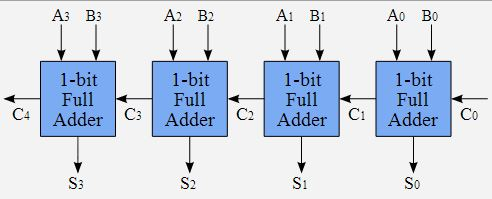
\includegraphics[width=\linewidth]{rippleadd}
\begin{itemize}
\item Efficiency should always be done in reference to cost model.
\item Optimization only plays a part later, it should not interfere with synthesis or it could become counterproductive.
\item Cost models place a cost on a circuit. The best circuit is the one with the lowest cost.
\item Examples of cost models include number of components (not useful nowadays as we have integrated circuits) and path depth (for combinational circuits).
\item For k inputs. There are $2^k$ lines in its truth table and $2^{(2^k)}$ boolean functions of k inputs.
\item General logic gates (LUT). Important in reconfigurable circuits. p = lut2 (a,b,c,d) x y
\item Gate delay is the time it takes for a signal to become valid once it has reached the gate.
\item Difference between invalidity and incorrectness.
\item For each signal x in the circuit, the time at which x becomes stable is called t(x). This is the path depth of x
\item Inputs to x are denoted a I(x).
\item Gate delay of a gate = gate delay of previous gates and the gates own delay. \[ t(x) = d + \underset{y \in I(x)}{\text{max } t(y)} \]
\item Critical path depth is the maximum path depth of all of its outputs. This can be used to determine the 'speed' of the circuit.

\end{itemize}


\section*{Lecture 4}
\begin{itemize}
\item Hazards, incorrect output based on varying gate delays (ie and2 x (inv x) results in a 1 value while (inv x) suffers gate delay).
\item A sequential circuit may have flip flops and feedback loops.
\item Sequential circuits perform computations through time.
\item Flip-flip is basic memory (hydra def - dff :: Clocked a -> a -> a)
\item Clocked used a Bool is simply not rich enough.
\item Real systems have a reset mechanism to put flip-flips into a valid state.
\item System must ensure a valid flip-flip value (no mid-voltages).
\item Flip-flops update on clock tick. Output continuous but only updates when clock pulses 1.
\item Abstract clock and Physical clock differences. Abstract cannot exist in real life. Components treat a 0 to 1 transition as a tick.
\item Synchronous model is used to prvent hazards. It boasts simple behavior and satisfies some constraints.
\item Synchronous if:
\begin{enumerate}
\item Contains logic gates and flip flops.
\item Every flip flop is connected to a global clock.
\item Every clock tick reaches each flip flop at the same time.
\item Each feedback loop goes via a flip flop.
\item Inputs to a circuit remain stable during a clock cycle.
\end{enumerate}
\item The restrictions on this mean that you cannot do combinational logic on clock input, you cannot introduce state via combinational feedback loops, and the circuit may malfunction if inputs are not stable for long enough.
\item State can be created by using flip flops or feedback loops in combinational logic (difficult to reason).
\item A synchronous circuit is a sequential circuit that behaves like a finite state automation.
\item Synchronous trade off. Restricted design chouce but much easier to reason the circuit.
\item Clock is an implicit input (as all dffs have the same clock ALWAYS).
\item Clock tick is a point in time. Clock cycle is an interval.
\item Clock skew is when a clock tick does not reach flip flops at the same time (such as in a fanout or if there are longer wires etc). 
\item The floor plan of the clock is normally laid out well in advance. See example H-tree. Known as the clock distribution.
\end{itemize}
\begin{center}
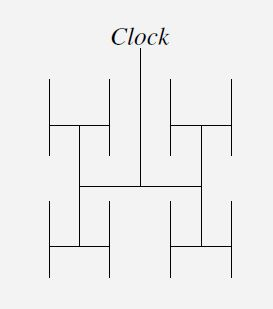
\includegraphics[width=0.5\linewidth]{hlayout}
\end{center}
\begin{itemize}
\item Circuits can have 'global' state in the synchronous model (values of all flip flops).
\item Circuit behaves as a single finite state automation.
\item Clock removes concern for intermediate values, hazards and gate delays (as they are all dealt with in the synchronous model).
\item reg1 component like a dff but with option ld signal that loads/ignores input value after clock tick accordingly.
\item reg1 works by multiplexing the input to a dff depending on the value of ld (obviously involves a feedback loop).
\end{itemize}


\section*{Lecture 5}
\begin{itemize}
\item list structure for words similar to haskell notation ie. (x:xs) = [a,b,c,d,e], x = a and b = [b,c,d,e]
\item equally the ++, !! and length operators can be used like in haskell.
\item field w i k takes the value of w starting at position i for k elements.
\item The type of a circuit describes its input. Such as how it's represented, how many inputs/outputs it takes/produces, parameter size and building blocks (if any).
\item You may use circuit generators to save making every component by hand. Eg. rippleAdd, a generic n-bit ripple adder that works for any word size.
\item This is not software to do the operation, it is still a real circuit.
\item Hydra has 4 'times'
\begin{enumerate}
\item Model Transformation Time
\item Circuit Generation Time
\item Simulator Compilation Time
\item Runtime
\end{enumerate}
\item Always use type a rather than Bool, its a hydra thing...
\item bitslice2 can be used so that [a] -> [a] -> [(a,a)]
\item mux1w is like a multiplexor but outputs words rather than single bits.
\item general n-bit reg an wlatch (wlatch doesn't take a load signal).
\item Modern RISC and CISC architectures use an indexed set of registers R0, R1, R2 etc which are implemented in a circuit called the register file.
\item Memory locations are usually bytes while registers contain words. Registers are few in comparison to memory (but much faster).
\item A dual-port register file provides separate input from output. Some register files have three ports (one in and 2 out).
\item How to handle address inputs. A tree of multiplexors and demultiplexors is needed for the addresses.
\item Look over register file recursive definitions.
\end{itemize}



\section*{Lecture 6}
\begin{itemize}
\item A test bench takes readable input and produces readable output. It converts to and from the actual signals and formats the output.
\item Lots of hydra test bench definitions. 'getbit', 'getbin' and 'gettc'
\item Additional hydra functions 'fanout', 'shl', 'bitslice2', 'orw'
\item An ALU is a combinational circuit. It is typically an adder with augmented functions to support other functions (eg bit shifting, subtraction, incrementing).
\item The critical path of the ALU should be very small.
\item Multiplication, division etc are performed over a series of clock ticks (by using sequential algorithms).
\item Sequential functions may operate as a machine language program, using normal processing registers or using a dedicated sequential circuit with its own registers (functional unit).
\item A functional unit is a sequential black box circuit with its own specific registers to perform a task like multiplication. It receives an input start and outputs an output signal 'ready'.
\item By using a functional unit (which is sequential), we can accept it may take a few clock cycles which means the global clock doesn't have to be slowed down.
\item If it were done by combinational logic the path depth would be so great the clock speed would have to be slowed down.
\item Use the shift and add algorithm to do multiplication. The inputs to x*y would be x y and start, the outputs would the be result and ready.

\end{itemize}



\section*{Lecture 7}
\begin{itemize}
\item Number of patterns in combinational logic; sum of cases, truth tables, fold, scan, map.
\item Design patterns are higher order functions. They take one or more circuit specifications as parameters.
\item The pattern defines how to connect up these given circuits in a regular pattern.
\item Pattern definition similar to ordinary circuit specification except that: It uses recursion to decompose groups of signals, it uses abstract circuits, rather than specific circuits, its type may include building block circuits.
\item map, map2, mapn used as in haskell.
\item fold as well. and2/or2 operate by using left folds.
\item ascanr is like fold but returns a list (including all intermediate values

\end{itemize}



\section*{Lecture 8}
\begin{itemize}
\item FSA (finite state automation) has a set of states, a stream of inputs (and state conversion function). It is used to recognize if the grammar of an input is correct.
\item FSAs need to be more general for practical applications. For example the new state transition function could produce a new output as well as defining a new state to enter.
\item In an unencoded representation you could use a dff for each state. If exactly one flip flop contains a 1 then it is in that state.
\item In an unencoded representation the no. of states = no. state flip flops.
\item In an encoded representation, each possible state is represented by a unique binary number held in a register.
\item In an encoded representation, $\text{no. of flip-flips} = \log_{2}(\text{no. of states})$
\item For the shift and add algorithm we must distinguish between what to put in the registers when start = 1 AND what to put in the registers when start $\neq$ 1 but a multiplication is still taking place.
\item When start = 1 x \& rx are both k bits, y i k bits, ry is 2k bits (it needs padding) and prod is 2k bits. rx and ry are set to the inputs on signals x \& y and prod is set to 0.
\item rx and ry are shifted right and left accordingly so that the algorithm is always examining the same bits.

\end{itemize}



\section*{Lecture 9}
\begin{itemize}
\item Sigma 16 is a 16-bit RISC style architecture. No bytes/words. Everything is 16-bit. 16 registers. Based on a simplified version of MIPS.
\item RRR format (two operands in the register file. The result goes into a register)
\item RX format (one operand is a register, the other is a memory address).
\item Memory addresses are constants, they are the combination of the displacement and the index/base.
\item RRR takes 4 inputs. The opcode op, destination d, and source addresses sa \& sb.
\item RX takes 4 inputs. The RX opcode (MUST be f), a destination register d, an index register sa and the secondary opcode sb.
\item RRR (one word) RX (two words, 4 4 bit fields and a 16-bit displacement).
\item Instructions can often be implemented without a feedback loop.
\end{itemize}
\begin{center}
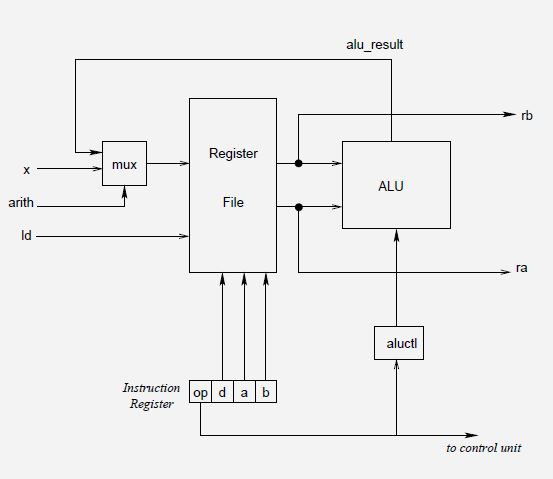
\includegraphics[width=\linewidth]{rtm}
\end{center}
\begin{itemize}
\item The datapath contains the combinational logic for calculations.
\item The control generates all of the control signals needed for the datapath
\item Similar design complexities, the datapath focuses more on structure whereas the control focuses on behavior.
\item Different design techniques (datapath designed directly as a circuit, control as an algorithm). The separation helps clarify timing.
\item Design of the datapath (all the logic and registers needed for calculations) will logically create a set of control signals that operate it.
\item There is a naming convention for control signals. ctl, subsystem, specific. Eg ctl\_rf\_ld.
\item The datapath contains registers, computational systems and interconnections.
\item It has two inputs, the control signals and a data word (from either memory system or the DMA input controller).
\item It outputs the bus to memory an I/O (it also outputs the states of the registers).
\item The datapath can be broken down into further subsystems (registers, ALU, busses etc).
\item Introduce an instruction register and program counter. For RX instructions an adr register is needed for the second word
\end{itemize}


\section*{Lecture 10}
\begin{itemize}
\item adr, pc and ir needed in the datapath to keep track of program execution. ALU needed to perform arithmetic.
\item The datapath contains the processor's rigiters. 
\item Aim 
\end{itemize}

\section*{Lecture 13}
\begin{itemize}
\item Latency is the time required for an operation. There is memory, instruction and communication latency.
\item Throughput is the amount of work performed per unit of time (eg. memory accesses per second).
\item For overall performance throughput is important.
\item For (re)solving bottlenecks, latency is often important.
\item Amdahl's law observes that the total speed up of the system may be less than the speed up of a part of the system depending on how much time is spend in said part of the system.
\item Example of Amdahl's law. If part A of a system can be sped up from 30s to 15s and is 30\% of the system process (the other part takes 70s) then the increase is 85s/100s which is 1.17 overall speed up factor.
\item Moore's law observes manufacturing trends. It states that the number of transistors per chip will double every two years (or some other number of years). 
\item Moore's law is based on the fact that integrated circuit fabrication technology makes gradual improvements which allows more components to be placed on chips.
\item Moore's law is not about speed. It is about chip density. The only way to increase speed now is to add more processing cores to a chip.
\item Performance should only really be measured in terms of its 'wall clock' time to run a piece of software.

\[  T = \text{ni} \cdot \text{cpi} \cdot \text{spc} \]
\[or\]
\[ T = \frac{\text{ni} \cdot \text{cpi}}{\text{cps}} \]

\item Where T = execution time in seconds, ni = no. instructions in order to execute the program, cpi = average no. clock cycles per instruction, spc = seconds per clock cycle, cps = cycles per second.
\item Reducing one of these factors does not necessarily reduce T.
\item In practice, the critical path will be the path from a register in a register file, through the ALU and back to the register file.
\item The M1 control algorithm will place whatever value is on the memory bus into the destination register. Even if the value is incorrect (for instance if it takes several clock cycles to compute).
\item More sophisticated solutions include using pipelining stages, interleaved memory and superscalar memory.
\item The M1 circuit has no interrupts, memory protection or virtual memory. No concurrency. Long-running instructions must execute until completion while the rest of the processor waits.
\item Pipelining is the application of parallelism to the steps in executing an instruction.
\item The basic application of pipelining is to 
\end{itemize}

\end{document}






















